
\documentclass[11pt,a4paper]{article}

\usepackage[a4paper,margin=2.2cm]{geometry}
\usepackage{fontspec}
\setmainfont{DejaVu Serif}
\setsansfont{DejaVu Sans}
\setmonofont{DejaVu Sans Mono}
\usepackage{graphicx}
\usepackage{booktabs}
\usepackage{tabularx}
\usepackage{longtable}
\usepackage{array}
\usepackage{float}
\usepackage{xcolor}
\usepackage{enumitem}
\usepackage{titlesec}
\usepackage{fancyhdr}
\usepackage{hyperref}
\usepackage{caption}
\usepackage{listings}
\usepackage{setspace}
\usepackage{ragged2e}
\usepackage{pdflscape}
\usepackage{multirow}
\usepackage{amsmath}

\definecolor{brandgreen}{HTML}{2F7D62}
\definecolor{softgreen}{HTML}{E9F3EF}
\definecolor{darktext}{HTML}{1F2937}
\definecolor{muted}{HTML}{6B7280}
\definecolor{lightline}{HTML}{D9E5E0}
\definecolor{codebg}{HTML}{F7F8FA}

\hypersetup{
    colorlinks=true,
    linkcolor=brandgreen,
    urlcolor=brandgreen,
    citecolor=brandgreen,
    pdftitle={E-Commerce Sales & Customer Retention Analytics Report},
    pdfauthor={Pham Dinh Duoc}
}

\pagestyle{fancy}
\fancyhf{}
\lhead{\sffamily E-Commerce Sales \& Customer Retention}
\rhead{\sffamily Technical Report}
\cfoot{\thepage}
\renewcommand{\headrulewidth}{0.4pt}

\titleformat{\section}
  {\sffamily\Large\bfseries\color{brandgreen}}
  {\thesection}{0.7em}{}
\titleformat{\subsection}
  {\sffamily\large\bfseries\color{darktext}}
  {\thesubsection}{0.7em}{}
\titleformat{\subsubsection}
  {\sffamily\normalsize\bfseries\color{darktext}}
  {\thesubsubsection}{0.7em}{}

\captionsetup{font=small,labelfont=bf}
\setlist[itemize]{leftmargin=1.2em,itemsep=0.25em,topsep=0.25em}
\setlist[enumerate]{leftmargin=1.5em,itemsep=0.25em,topsep=0.25em}
\renewcommand{\arraystretch}{1.25}
\setlength{\parskip}{0.55em}
\setlength{\parindent}{0pt}
\onehalfspacing
\sloppy

\lstdefinestyle{code}{
  backgroundcolor=\color{codebg},
  basicstyle=\ttfamily\footnotesize,
  breaklines=true,
  frame=single,
  rulecolor=\color{lightline},
  columns=fullflexible,
  keepspaces=true
}
\lstset{style=code}

\newcommand{\kpi}[2]{\textbf{#1} & #2 \\}
\newcommand{\sourceNote}[1]{\vspace{-0.4em}\caption*{\footnotesize\color{muted}Nguồn: #1}}

\begin{document}

\begin{titlepage}
\pagecolor{softgreen}
\centering
\vspace*{1.5cm}
{\sffamily\bfseries\Huge\color{brandgreen} E-Commerce Sales \& Customer Retention Analytics\par}
\vspace{0.4cm}
{\sffamily\Large Technical Report for Data Analyst Intern Challenge\par}
\vspace{1.2cm}
\rule{0.78\textwidth}{1pt}
\vspace{1.0cm}

\begin{tabular}{rl}
\textbf{Candidate} & Phạm Đình Được \\
\textbf{Project track} & Retail \& Marketing Analytics \\
\textbf{Tools} & SQL, Python, Tableau, Data Storytelling \\
\textbf{Main output} & Tableau dashboard + reproducible RFM pipeline \\
\textbf{Report date} & \today \\
\end{tabular}

\vfill
\begin{minipage}{0.82\textwidth}
\centering
\textit{Mục tiêu của báo cáo là chuyển dữ liệu giao dịch e-commerce thành insight kinh doanh có thể hành động: doanh thu đến từ đâu, khách hàng nào tạo giá trị cao, nhóm nào có rủi ro churn, và doanh nghiệp nên ưu tiên retention như thế nào.}
\end{minipage}
\vfill
\end{titlepage}
\nopagecolor

\tableofcontents
\newpage

\section{Executive Summary}

Dự án phân tích dữ liệu bán lẻ trực tuyến bằng hai nhóm dữ liệu chính: dữ liệu giao dịch và bảng RFM segmentation. Mục tiêu là theo dõi hiệu suất doanh thu, nhận diện nhóm khách hàng giá trị cao và đề xuất chiến lược giữ chân khách hàng dựa trên hành vi mua hàng.

\begin{table}[H]
\centering
\caption{KPI tổng quan của dự án}
\begin{tabular}{ll}
\toprule
\textbf{KPI} & \textbf{Giá trị} \\
\midrule
\kpi{Total Sales}{\$ 8,911,407.90}
\kpi{Total Orders}{18,532}
\kpi{Average Order Value}{\$ 480.87}
\kpi{Total Customers}{4,338}
\kpi{Active Customers}{3,473}
\kpi{Churned Customers}{865}
\kpi{Churn Rate}{19.94\%}
\bottomrule
\end{tabular}
\end{table}

\textbf{Kết luận chính:}
\begin{itemize}
    \item Doanh thu đạt \textbf{\$ 8.91M} với \textbf{18,532} đơn hàng và \textbf{4,338} khách hàng.
    \item Q4/2024 đóng góp \textbf{35.39\%} tổng doanh thu, phản ánh tính mùa vụ rõ rệt ở giai đoạn cuối năm.
    \item United Kingdom chiếm \textbf{82.01\%} doanh thu, cho thấy mức độ phụ thuộc thị trường rất cao.
    \item Nhóm \textbf{High-Value} chiếm khoảng \textbf{20.01\%} khách hàng nhưng đóng góp \textbf{74.62\%} doanh thu.
    \item Churn Rate ở mức \textbf{19.94\%}. Phần lớn khách churned có doanh thu thấp, nhưng vẫn tồn tại nhóm High-Value đã churn với tổng Monetary khoảng \textbf{\$ 229K}, cần ưu tiên win-back.
\end{itemize}

\section{Business Context}

\subsection{Vấn đề kinh doanh}

Bài toán không chỉ là theo dõi doanh thu. Với e-commerce, doanh nghiệp cần trả lời bốn câu hỏi quản trị:

\begin{enumerate}
    \item Doanh thu đang tăng hay giảm theo thời gian?
    \item Tăng trưởng đến từ số lượng đơn hàng hay giá trị trung bình mỗi đơn hàng?
    \item Thị trường, sản phẩm và nhóm khách hàng nào đang tạo doanh thu chính?
    \item Nhóm khách hàng nào có nguy cơ rời bỏ và nên được ưu tiên remarketing?
\end{enumerate}

Vì vậy, dự án được định vị theo track \textbf{Retail \& Marketing Analytics}. Dashboard cần hỗ trợ quyết định ngân sách marketing, retention campaign và chiến lược mở rộng thị trường.

\subsection{Business Objectives}

\begin{tabularx}{\textwidth}{p{3.6cm}X}
\toprule
\textbf{Mục tiêu} & \textbf{Ý nghĩa phân tích} \\
\midrule
Theo dõi hiệu suất kinh doanh & Đo Sales, Orders, AOV, Active Customers và Churn Rate để nắm tình hình tổng quan. \\
Phân tích tăng trưởng & Tách doanh thu thành hai driver: số lượng đơn và giá trị trung bình mỗi đơn. \\
Xác định nguồn doanh thu & Tìm quốc gia, sản phẩm và segment đóng góp chính. \\
Tối ưu retention & Dùng RFM để phân loại Champions, Loyal, New, At Risk và Lost Customers. \\
Đề xuất hành động & Chuyển insight thành campaign: VIP, win-back, cross-sell, second-order incentive. \\
\bottomrule
\end{tabularx}

\section{Dataset Overview}

Dữ liệu đã qua xử lý gồm hai file đầu ra dành cho Tableau:

\begin{itemize}
    \item \texttt{tableau\_transactions\_final.csv}: dữ liệu giao dịch, gồm InvoiceNo, Sales, InvoiceDate, Quantity, UnitPrice, CustomerID, Country, Status và Is\_Top\_20.
    \item \texttt{tableau\_rfm\_segmentation.csv}: dữ liệu cấp khách hàng, gồm Recency, Frequency, Monetary, R\_Score, F\_Score, M\_Score, Status và Is\_Top\_20.
\end{itemize}

\begin{table}[H]
\centering
\caption{Tóm tắt dữ liệu đầu vào sau xử lý}
\begin{tabular}{lr}
\toprule
\textbf{Chỉ tiêu} & \textbf{Giá trị} \\
\midrule
Số dòng transaction & 397,884 \\
Số đơn hàng duy nhất & 18,532 \\
Số khách hàng duy nhất & 4,338 \\
Số quốc gia & 37 \\
Số sản phẩm duy nhất & 3,877 \\
Khoảng thời gian & 2024-01-01 đến 2025-01-09 \\
\bottomrule
\end{tabular}
\end{table}

\subsection{Data Pipeline}

Pipeline được thiết kế để có thể tái chạy từ raw data tới dữ liệu Tableau-ready. Cấu trúc source code nên chia thành bốn module:

\begin{lstlisting}[language=bash]
src/
├── data_cleaning.py          # Load raw data, clean transaction, create Sales
├── rfm_segmentation.py       # Calculate RFM, scores, segments, churn status
├── generate_tableau_data.py  # Merge RFM into transactions and export CSV
└── main.py                   # Run full pipeline
\end{lstlisting}

Luồng xử lý đề xuất:

\begin{center}
\fbox{\begin{minipage}{0.88\textwidth}
Raw CSV $\rightarrow$ SQL validation $\rightarrow$ Python cleaning $\rightarrow$ RFM scoring $\rightarrow$ Tableau CSV export $\rightarrow$ Dashboard $\rightarrow$ Business recommendation
\end{minipage}}
\end{center}

\section{Data Cleaning and Feature Engineering}

\subsection{Quy tắc làm sạch dữ liệu}

Các bước xử lý chính:

\begin{enumerate}
    \item Chuẩn hóa kiểu dữ liệu: \texttt{InvoiceDate} sang datetime, \texttt{Quantity} và \texttt{UnitPrice} sang numeric.
    \item Loại bỏ các dòng thiếu \texttt{InvoiceNo}, \texttt{InvoiceDate}, \texttt{CustomerID}, \texttt{Quantity} hoặc \texttt{UnitPrice}.
    \item Loại bỏ hóa đơn hủy, thường có \texttt{InvoiceNo} bắt đầu bằng ký tự \texttt{C}.
    \item Loại bỏ transaction có \texttt{Quantity <= 0} hoặc \texttt{UnitPrice <= 0}.
    \item Tạo biến \texttt{Sales = Quantity * UnitPrice}.
    \item Chuẩn hóa \texttt{Description} và \texttt{Country} để phục vụ dashboard.
\end{enumerate}

\subsection{Các chỉ số được tạo mới}

\begin{table}[H]
\centering
\caption{Feature engineering phục vụ phân tích}
\begin{tabularx}{\textwidth}{p{3.5cm}p{5cm}X}
\toprule
\textbf{Field} & \textbf{Công thức / logic} & \textbf{Mục đích} \\
\midrule
Sales & Quantity $\times$ UnitPrice & Doanh thu cấp transaction. \\
AOV & Total Sales / COUNTD(InvoiceNo) & Đo giá trị trung bình của mỗi đơn hàng. \\
Recency & Snapshot Date - Last Purchase Date & Đo số ngày từ lần mua gần nhất. \\
Frequency & COUNTD(InvoiceNo) theo CustomerID & Đo tần suất mua hàng. \\
Monetary & SUM(Sales) theo CustomerID & Đo tổng giá trị đóng góp của khách hàng. \\
Status & Active nếu Recency $\le$ churn threshold, ngược lại Churned & Phân loại khách còn hoạt động hay đã rời bỏ. \\
Is\_Top\_20 & Monetary thuộc top 20\% & Nhận diện khách hàng giá trị cao. \\
\bottomrule
\end{tabularx}
\end{table}

\section{RFM Segmentation Methodology}

\subsection{Khái niệm RFM}

RFM là phương pháp phân tích khách hàng dựa trên ba biến hành vi:

\begin{itemize}
    \item \textbf{Recency}: khách hàng mua gần đây đến mức nào. Recency càng thấp càng tốt.
    \item \textbf{Frequency}: khách hàng mua thường xuyên đến mức nào. Frequency càng cao càng tốt.
    \item \textbf{Monetary}: khách hàng đóng góp doanh thu bao nhiêu. Monetary càng cao càng tốt.
\end{itemize}

Điểm R, F, M được chia thành thang 1-5. Với Recency, khách hàng có Recency thấp được gán R\_Score cao. Với Frequency và Monetary, giá trị càng cao thì điểm càng cao.

\subsection{Logic đặt Segment Name}

\begin{lstlisting}[language=Python]
IF R_Score >= 4 AND F_Score >= 4 AND M_Score >= 4 THEN "Champions"
ELSEIF R_Score >= 4 AND F_Score >= 3 AND M_Score >= 3 THEN "Loyal Customers"
ELSEIF R_Score >= 4 AND F_Score <= 2 THEN "New Customers"
ELSEIF R_Score <= 2 AND F_Score >= 4 AND M_Score >= 4 THEN "At Risk High Value"
ELSEIF R_Score <= 2 AND F_Score >= 3 THEN "At Risk"
ELSEIF R_Score <= 2 AND F_Score <= 2 THEN "Lost Customers"
ELSE "Standard"
END
\end{lstlisting}

\subsection{Ý nghĩa kinh doanh của từng segment}

\begin{tabularx}{\textwidth}{p{3.6cm}X}
\toprule
\textbf{Segment} & \textbf{Diễn giải} \\
\midrule
Champions & Mua gần đây, mua thường xuyên và chi tiêu cao. Đây là nhóm cần giữ chân ưu tiên nhất. \\
Loyal Customers & Mua gần đây, tần suất tương đối tốt, có tiềm năng upsell/cross-sell. \\
New Customers & Mới mua gần đây nhưng tần suất thấp. Cần khuyến khích đơn hàng thứ hai. \\
At Risk High Value & Từng mua nhiều và chi tiêu cao nhưng đã lâu chưa quay lại. Cần win-back khẩn cấp. \\
At Risk & Có dấu hiệu giảm tương tác, cần remarketing hoặc ưu đãi phù hợp. \\
Lost Customers & Lâu chưa quay lại và tần suất thấp. Chỉ nên dùng chiến dịch chi phí thấp. \\
Standard & Nhóm trung bình, cần nuôi dưỡng bằng khuyến mãi định kỳ. \\
\bottomrule
\end{tabularx}

\section{Dashboard Design Review}

Dashboard gồm các khối quan trọng: KPI cards, Sales Trend, Orders vs AOV, Top Country, Top Products, Churn Comparison, RFM Heatmap, Frequency vs Monetary, Sales by Segment và bảng phân tích theo Status/Segment.

\begin{figure}[H]
\centering
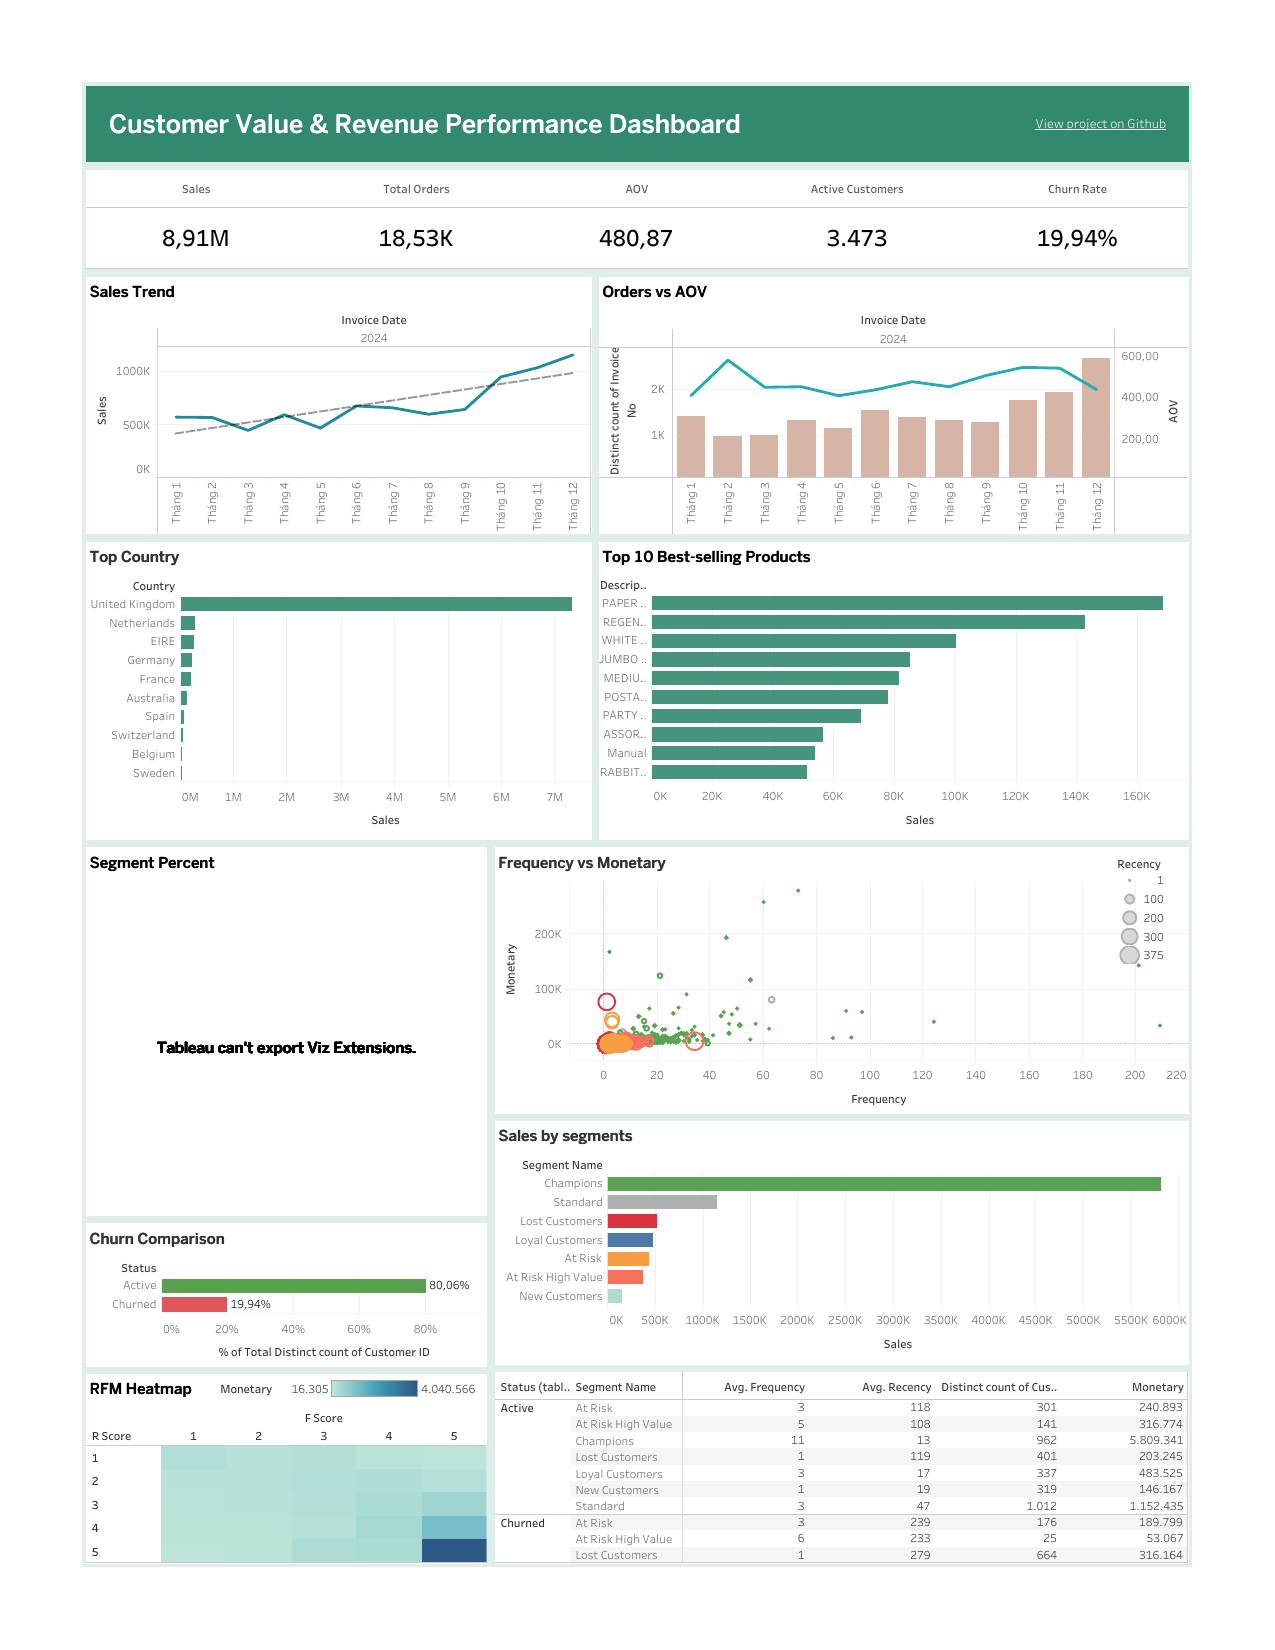
\includegraphics[width=0.95\textwidth]{figures/dashboard_render/page-1.png}
\caption{Ảnh dashboard hiện tại được export từ Tableau}
\sourceNote{Dashboard PDF hiện tại}
\end{figure}

\subsection{Mục tiêu Dashboard}

\begin{itemize}
    \item Có đủ tầng phân tích giúp người xem có cái nhìn tổng quan tới chi tiết: revenue, market, product, customer status, RFM.
    \item KPI cards đặt ở đầu giúp người xem nắm nhanh health check của business.
    \item Orders vs AOV là biểu đồ tốt vì giúp giải thích doanh thu tăng do volume hay do giá trị đơn hàng.
    \item RFM Heatmap và Frequency vs Monetary giúp hỗ trợ customer analytics.
\end{itemize}

% \subsection{Điểm cần sửa trước khi nộp}

% \begin{enumerate}
%     \item \textbf{Segment Percent bị lỗi export}: trong PDF có dòng \texttt{Tableau can't export Viz Extensions}. Nên thay bằng native bar chart hoặc donut chart không dùng extension.
%     \item \textbf{Title chart cần chuẩn hóa}: đổi \texttt{Top Country} thành \texttt{Top Countries by Sales}, \texttt{Sales by segments} thành \texttt{Sales by Customer Segment}.
%     \item \textbf{Bảng cuối cần biến thành Action Table}: thêm cột Business Action để thể hiện recommendation.
%     \item \textbf{Thêm Recommendation Panel}: đặt cuối dashboard để nêu rõ hành động cho từng segment.
%     \item \textbf{Giữ màu segment nhất quán}: Champions xanh, Loyal xanh dương, New xanh ngọc, Standard xám, At Risk cam, Lost đỏ.
% \end{enumerate}

\section{Detailed Analysis}

\subsection{Revenue Performance}

\begin{figure}[H]
\centering
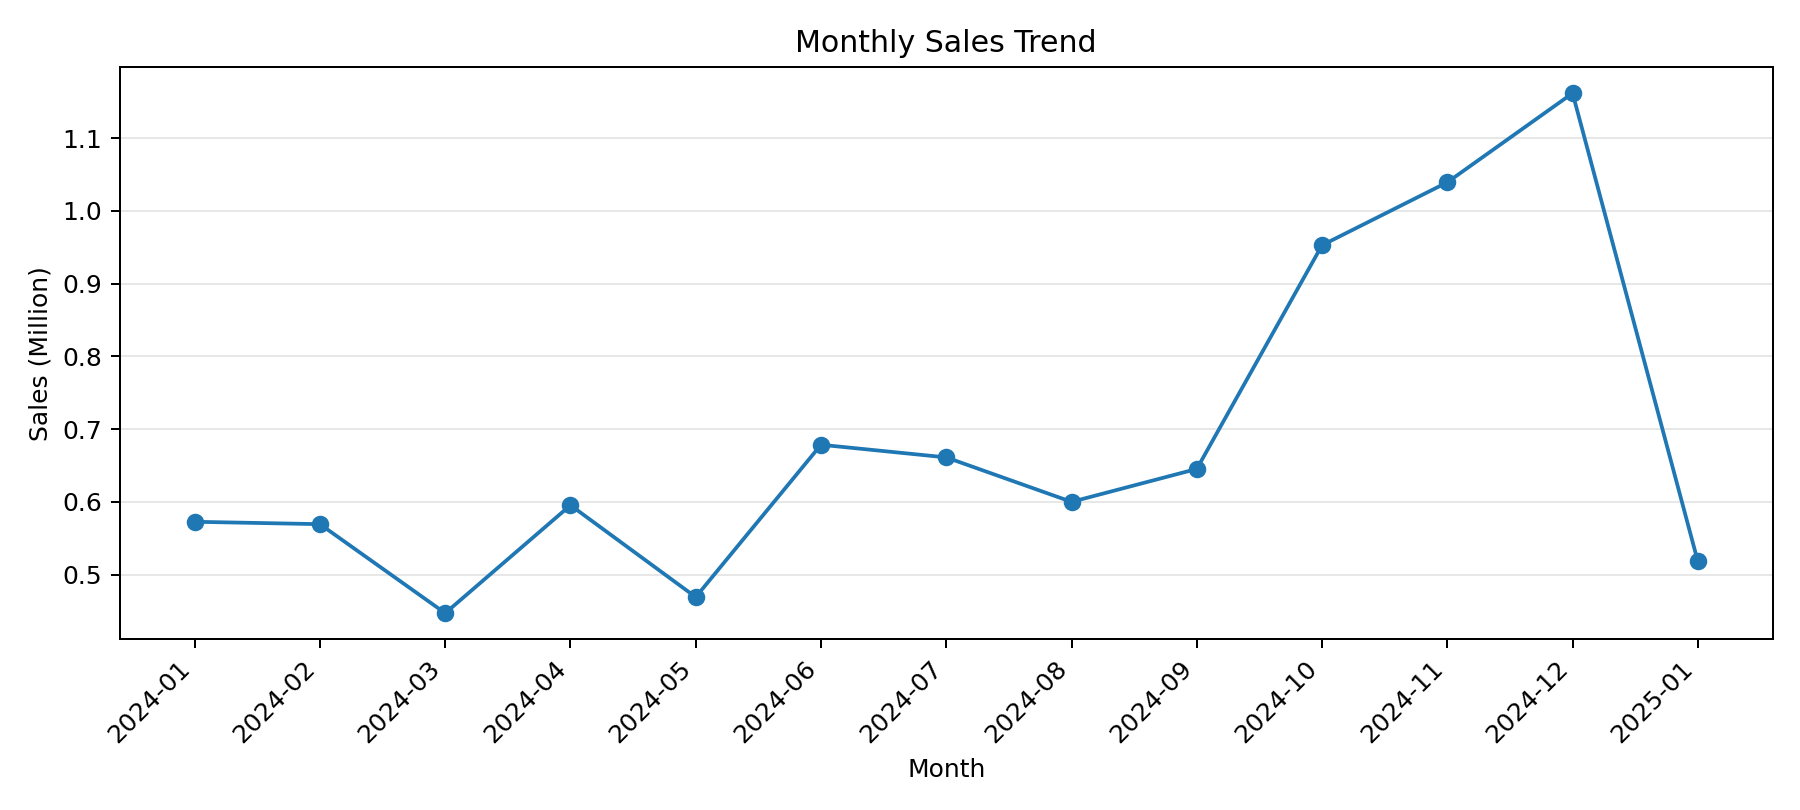
\includegraphics[width=0.92\textwidth]{figures/monthly_sales.png}
\caption{Xu hướng doanh thu theo tháng}
\sourceNote{Tính toán từ \texttt{tableau\_transactions\_final.csv}}
\end{figure}

Doanh thu có xu hướng tăng mạnh từ tháng 10/2024 đến tháng 12/2024. Tháng có doanh thu cao nhất là \textbf{2024-12} với \textbf{\$ 1.16M}, chiếm \textbf{13.04\%} tổng doanh thu. Giai đoạn Q4/2024 đóng góp \textbf{35.39\%} doanh thu toàn kỳ, cho thấy tính mùa vụ rõ rệt.

\begin{longtable}{lrrrr}
\caption{Monthly sales, orders, AOV và MoM growth}\\
\toprule
\textbf{Month} & \textbf{Sales} & \textbf{Orders} & \textbf{AOV} & \textbf{MoM} \\
\midrule
\endfirsthead
\toprule
\textbf{Month} & \textbf{Sales} & \textbf{Orders} & \textbf{AOV} & \textbf{MoM} \\
\midrule
\endhead
2024-01 & 0.57M & 1,400 & 409.08 & - \\
2024-02 & 0.57M & 987 & 576.95 & -0.6\% \\
2024-03 & 0.45M & 997 & 448.48 & -21.5\% \\
2024-04 & 0.60M & 1,321 & 450.80 & 33.2\% \\
2024-05 & 0.47M & 1,149 & 408.36 & -21.2\% \\
2024-06 & 0.68M & 1,555 & 436.40 & 44.6\% \\
2024-07 & 0.66M & 1,393 & 474.67 & -2.6\% \\
2024-08 & 0.60M & 1,331 & 450.86 & -9.2\% \\
2024-09 & 0.65M & 1,280 & 504.17 & 7.5\% \\
2024-10 & 0.95M & 1,755 & 542.93 & 47.6\% \\
2024-11 & 1.04M & 1,929 & 538.79 & 9.1\% \\
2024-12 & 1.16M & 2,657 & 437.27 & 11.8\% \\
2025-01 & 0.52M & 778 & 666.06 & -55.4\% \\
\bottomrule
\end{longtable}

\textbf{Insight:} doanh thu tăng mạnh nhất ở tháng 10/2024, tăng khoảng \textbf{47.6\%} so với tháng 9/2024. Từ tháng 1/2024 tới tháng 12/2024, doanh thu tăng hơn \textbf{102.9\%}. Tuy nhiên tháng 1/2025 giảm \textbf{55.4\%} so với tháng 12/2024, phản ánh hiệu ứng sau mùa cao điểm hoặc dữ liệu tháng 1 chưa đầy đủ.

\subsection{Orders vs AOV}

\begin{figure}[H]
\centering
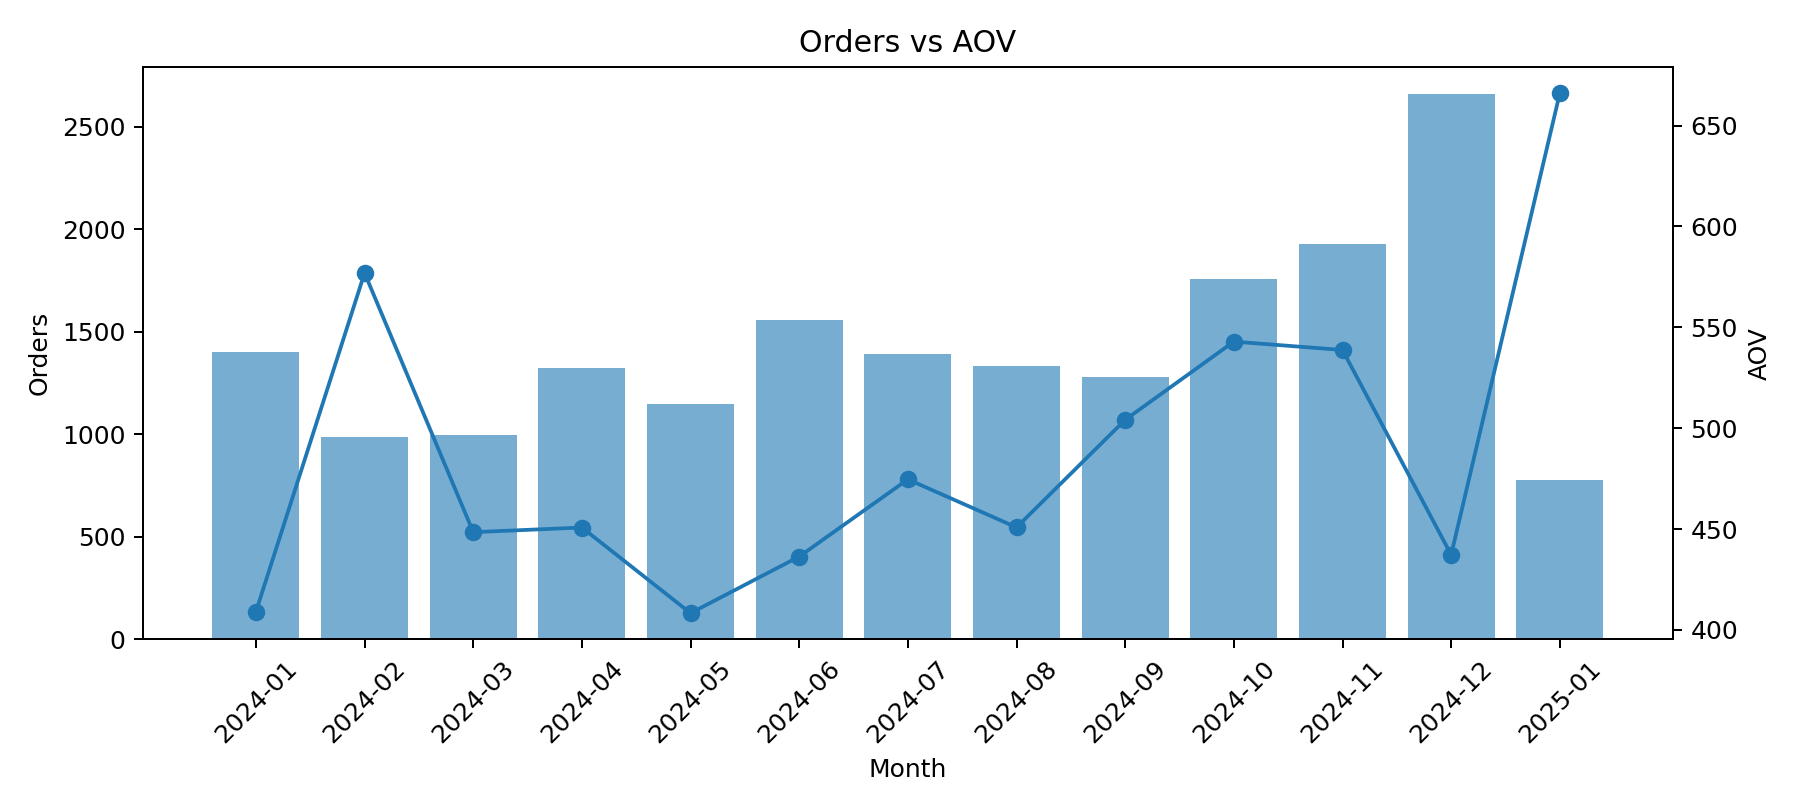
\includegraphics[width=0.92\textwidth]{figures/orders_vs_aov.png}
\caption{Số đơn hàng và AOV theo tháng}
\sourceNote{Tính toán từ \texttt{tableau\_transactions\_final.csv}}
\end{figure}

Biểu đồ Orders vs AOV giúp tách doanh thu thành hai driver:

\begin{itemize}
    \item Nếu Orders tăng và AOV tăng: tăng trưởng khỏe.
    \item Nếu Orders tăng nhưng AOV giảm: doanh thu tăng chủ yếu nhờ volume, có thể do khuyến mãi hoặc đơn hàng nhỏ.
    \item Nếu Orders giảm nhưng AOV tăng: doanh nghiệp có ít đơn hơn nhưng giá trị đơn cao hơn.
    \item Nếu cả Orders và AOV đều giảm: tín hiệu xấu cần xử lý.
\end{itemize}

Tháng 12/2024 có doanh thu cao nhất với \textbf{2,657} đơn nhưng AOV không cao nhất. Tháng 1/2025 có AOV rất cao nhưng số đơn giảm mạnh, vì vậy không nên diễn giải tháng 1/2025 là tăng trưởng tốt nếu chỉ nhìn AOV.

\subsection{Market Performance}

\begin{figure}[H]
\centering
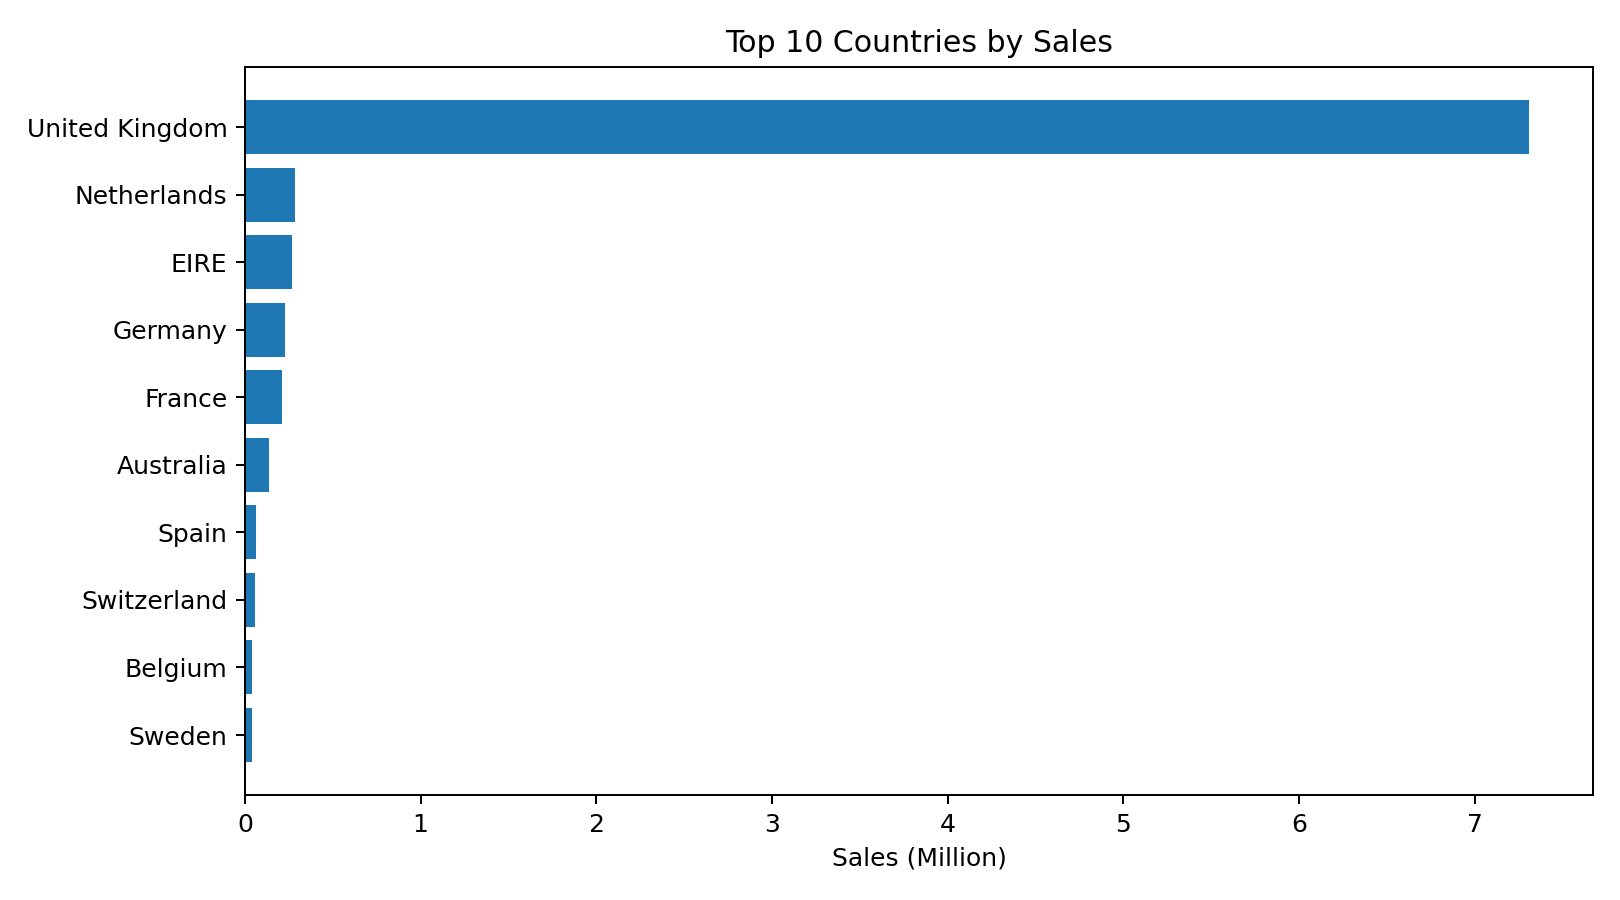
\includegraphics[width=0.88\textwidth]{figures/top_countries.png}
\caption{Top 10 quốc gia theo doanh thu}
\sourceNote{Tính toán từ \texttt{tableau\_transactions\_final.csv}}
\end{figure}

\begin{table}[H]
\centering
\caption{Top 10 countries by Sales}
\begin{tabular}{lrrrr}
\toprule
\textbf{Country} & \textbf{Sales} & \textbf{Share} & \textbf{Orders} & \textbf{Customers} \\
\midrule
United Kingdom & 7.31M & 82.01\% & 16,646 & 3,920 \\
Netherlands & 0.29M & 3.20\% & 94 & 9 \\
EIRE & 0.27M & 2.98\% & 260 & 3 \\
Germany & 0.23M & 2.57\% & 457 & 94 \\
France & 0.21M & 2.35\% & 389 & 87 \\
Australia & 0.14M & 1.55\% & 57 & 9 \\
Spain & 0.06M & 0.69\% & 90 & 30 \\
Switzerland & 0.06M & 0.63\% & 51 & 21 \\
Belgium & 0.04M & 0.46\% & 98 & 25 \\
Sweden & 0.04M & 0.43\% & 36 & 8 \\
\bottomrule
\end{tabular}
\end{table}

\textbf{Insight:} United Kingdom chiếm \textbf{82.01\%} doanh thu, trong khi top 5 quốc gia chiếm \textbf{93.11\%}. Đây là mức tập trung cao, có lợi khi doanh nghiệp hiểu rõ thị trường lõi nhưng cũng tạo rủi ro phụ thuộc.

\textbf{Action:} tiếp tục bảo vệ thị trường UK bằng loyalty/retention, đồng thời thử nghiệm campaign tại Germany, France, Netherlands và EIRE để giảm concentration risk.

\subsection{Product Performance}

\begin{table}[H]
\centering
\caption{Top 10 products by revenue}
\begin{tabular}{p{5.3cm}rrrr}
\toprule
\textbf{Product} & \textbf{Sales} & \textbf{Share} & \textbf{Quantity} & \textbf{Orders} \\
\midrule
PAPER CRAFT , LITTLE BIRDIE & 0.17M & 1.89\% & 80,995 & 1 \\
REGENCY CAKESTAND 3 TIER & 0.14M & 1.60\% & 12,402 & 1,703 \\
WHITE HANGING HEART T-LIGHT HOLDER & 0.10M & 1.13\% & 36,725 & 1,971 \\
JUMBO BAG RED RETROSPOT & 0.09M & 0.96\% & 46,181 & 1,600 \\
MEDIUM CERAMIC TOP STORAGE JAR & 0.08M & 0.91\% & 77,916 & 195 \\
POSTAGE & 0.08M & 0.87\% & 3,120 & 1,099 \\
PARTY BUNTING & 0.07M & 0.77\% & 15,291 & 1,379 \\
ASSORTED COLOUR BIRD ORNAMENT & 0.06M & 0.63\% & 35,362 & 1,375 \\
Manual & 0.05M & 0.60\% & 7,173 & 253 \\
RABBIT NIGHT LIGHT & 0.05M & 0.58\% & 27,202 & 801 \\
\bottomrule
\end{tabular}
\end{table}

Top 10 sản phẩm đóng góp khoảng \textbf{9.95\%} doanh thu. Sản phẩm đứng đầu là \textbf{PAPER CRAFT , LITTLE BIRDIE} với doanh thu \textbf{\$ 168.5K}. Tuy nhiên sản phẩm top 1 chỉ xuất hiện trong \textbf{1} đơn, nên cần kiểm tra đây là đơn bulk/B2B hay outlier.

\textbf{Action:}
\begin{itemize}
    \item Tách sản phẩm thành nhóm \textit{high revenue because of volume} và \textit{high revenue because of unit value}.
    \item Với sản phẩm tần suất đơn cao như \textit{WHITE HANGING HEART T-LIGHT HOLDER} hoặc \textit{REGENCY CAKESTAND 3 TIER}, nên dùng cho cross-sell/bundle.
    \item Với sản phẩm doanh thu cao nhưng ít đơn, cần kiểm tra tính ổn định trước khi dự báo tồn kho.
\end{itemize}

\subsection{Customer Status and Churn}

\begin{figure}[H]
\centering
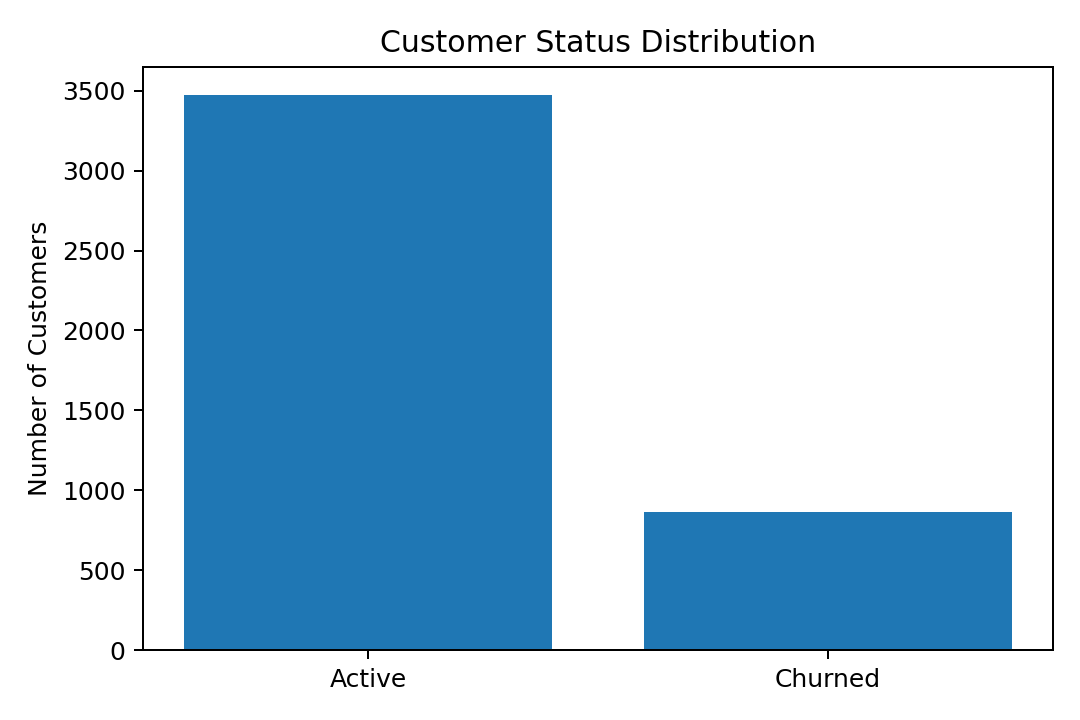
\includegraphics[width=0.62\textwidth]{figures/customer_status.png}
\caption{Phân bổ Active vs Churned customers}
\sourceNote{Tính toán từ \texttt{tableau\_rfm\_segmentation.csv}}
\end{figure}

\begin{table}[H]
\centering
\caption{Customer status summary}
\begin{tabular}{lrrrrrr}
\toprule
\textbf{Status} & \textbf{Customers} & \textbf{Cust. Share} & \textbf{Monetary} & \textbf{Rev. Share} & \textbf{Avg R} & \textbf{Avg F} \\
\midrule
Active & 3,473 & 80.06\% & 8.35M & 93.73\% & 49.2 & 5.0 \\
Churned & 865 & 19.94\% & 0.56M & 6.27\% & 269.5 & 1.5 \\
\bottomrule
\end{tabular}
\end{table}

\textbf{Insight:} Active customers chiếm \textbf{80.06\%} số khách và đóng góp \textbf{93.73\%} Monetary. Churned customers chiếm gần \textbf{19.94\%} số khách nhưng chỉ đóng góp \textbf{6.27\%} doanh thu. Điều này cho thấy churn phần lớn nằm ở nhóm giá trị thấp, nhưng vẫn cần ưu tiên xử lý nhóm High-Value đã churn.

\subsection{Customer Segmentation}

\begin{figure}[H]
\centering
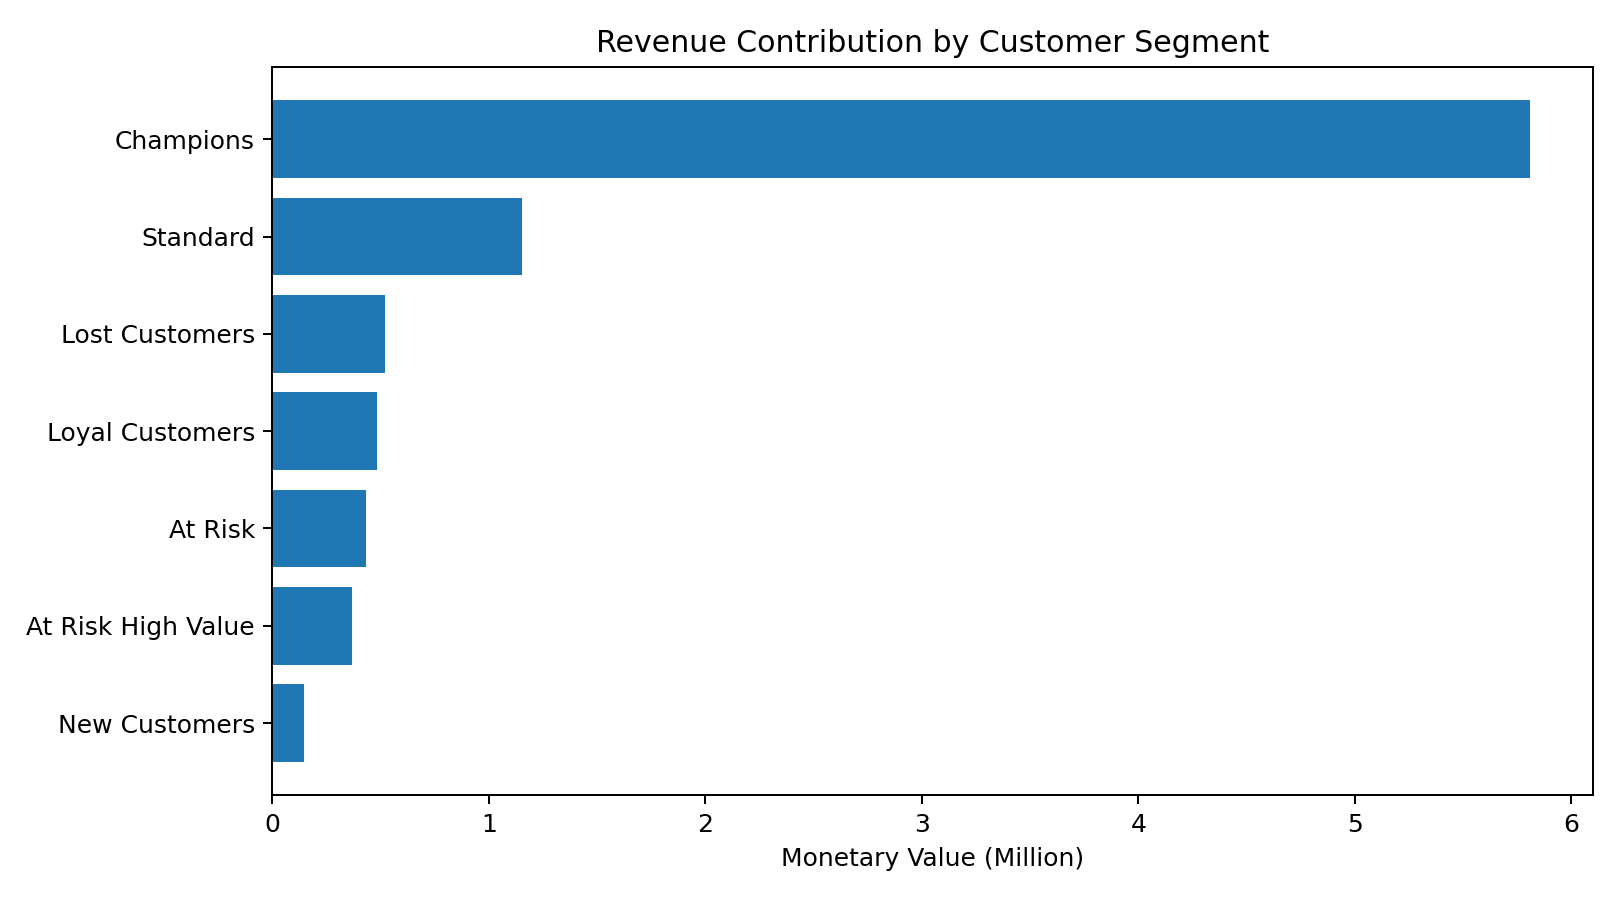
\includegraphics[width=0.88\textwidth]{figures/segment_revenue.png}
\caption{Doanh thu theo customer segment}
\sourceNote{Tính toán từ \texttt{tableau\_rfm\_segmentation.csv}}
\end{figure}

\begin{longtable}{lrrrrrr}
\caption{Segment summary}\\
\toprule
\textbf{Segment} & \textbf{Cust.} & \textbf{Cust. \%} & \textbf{Monetary} & \textbf{Rev. \%} & \textbf{Avg R} & \textbf{Avg F} \\
\midrule
\endfirsthead
\toprule
\textbf{Segment} & \textbf{Cust.} & \textbf{Cust. \%} & \textbf{Monetary} & \textbf{Rev. \%} & \textbf{Avg R} & \textbf{Avg F} \\
\midrule
\endhead
Champions & 962 & 22.18\% & 5.81M & 65.19\% & 13.4 & 11.1 \\
Standard & 1,012 & 23.33\% & 1.15M & 12.93\% & 47.0 & 3.0 \\
Lost Customers & 1,065 & 24.55\% & 0.52M & 5.83\% & 218.7 & 1.1 \\
Loyal Customers & 337 & 7.77\% & 0.48M & 5.43\% & 17.2 & 3.2 \\
At Risk & 477 & 11.00\% & 0.43M & 4.83\% & 162.8 & 2.7 \\
At Risk High Value & 166 & 3.83\% & 0.37M & 4.15\% & 126.6 & 5.5 \\
New Customers & 319 & 7.35\% & 0.15M & 1.64\% & 19.3 & 1.2 \\
\bottomrule
\end{longtable}

\textbf{Insight:} Champions chiếm \textbf{22.18\%} khách hàng nhưng đóng góp \textbf{65.19\%} doanh thu. Đây là nhóm có tần suất mua trung bình \textbf{11.1} đơn/khách và Recency trung bình chỉ \textbf{13.4} ngày. Doanh nghiệp nên ưu tiên bảo vệ nhóm này trước khi mở rộng ngân sách vào nhóm giá trị thấp.

\subsection{Top 20\% Customer Contribution}

\begin{figure}[H]
\centering
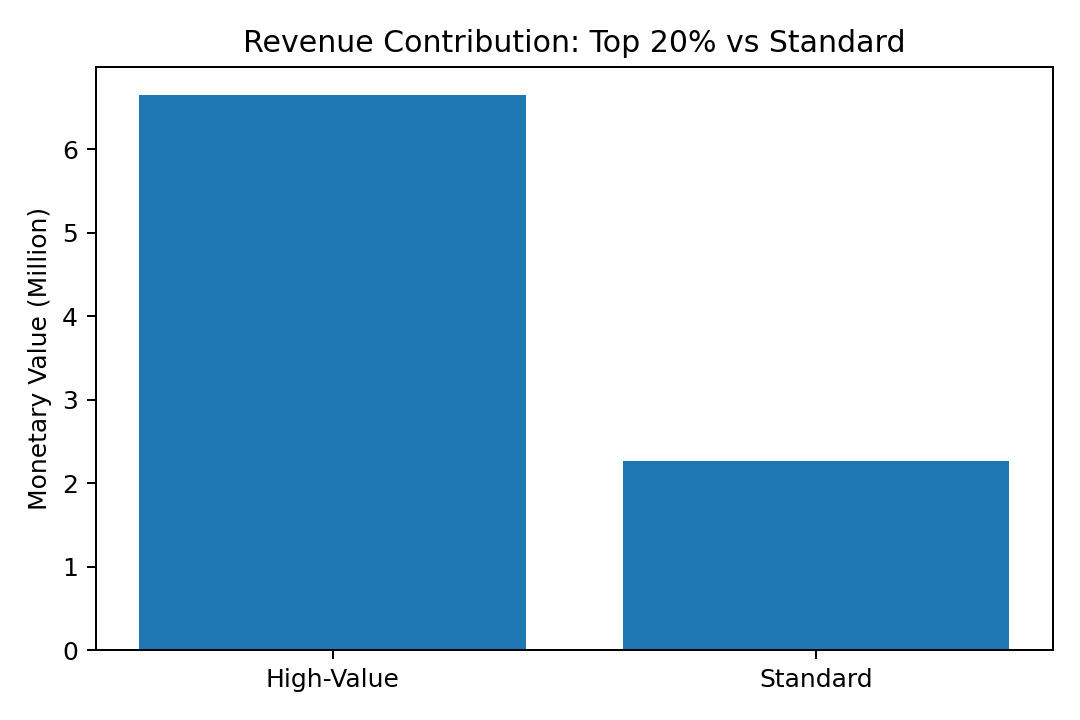
\includegraphics[width=0.62\textwidth]{figures/top20_contribution.png}
\caption{Đóng góp doanh thu của High-Value vs Standard customers}
\sourceNote{Tính toán từ \texttt{tableau\_rfm\_segmentation.csv}}
\end{figure}

\begin{table}[H]
\centering
\caption{Top 20\% customer contribution}
\begin{tabular}{lrrrr}
\toprule
\textbf{Group} & \textbf{Customers} & \textbf{Cust. Share} & \textbf{Monetary} & \textbf{Rev. Share} \\
\midrule
High-Value & 868 & 20.01\% & 6.65M & 74.62\% \\
Standard & 3,470 & 79.99\% & 2.26M & 25.38\% \\
\bottomrule
\end{tabular}
\end{table}

\textbf{Insight đắt giá nhất:} khoảng \textbf{20\%} khách hàng tạo ra gần \textbf{75\%} doanh thu. Đây là bằng chứng rõ ràng rằng marketing budget không nên phân bổ đồng đều cho mọi khách hàng. Thay vào đó, nên ưu tiên retention cho High-Value customers vì đây là nhóm quyết định dòng tiền.

\subsection{RFM Heatmap}

\begin{figure}[H]
\centering
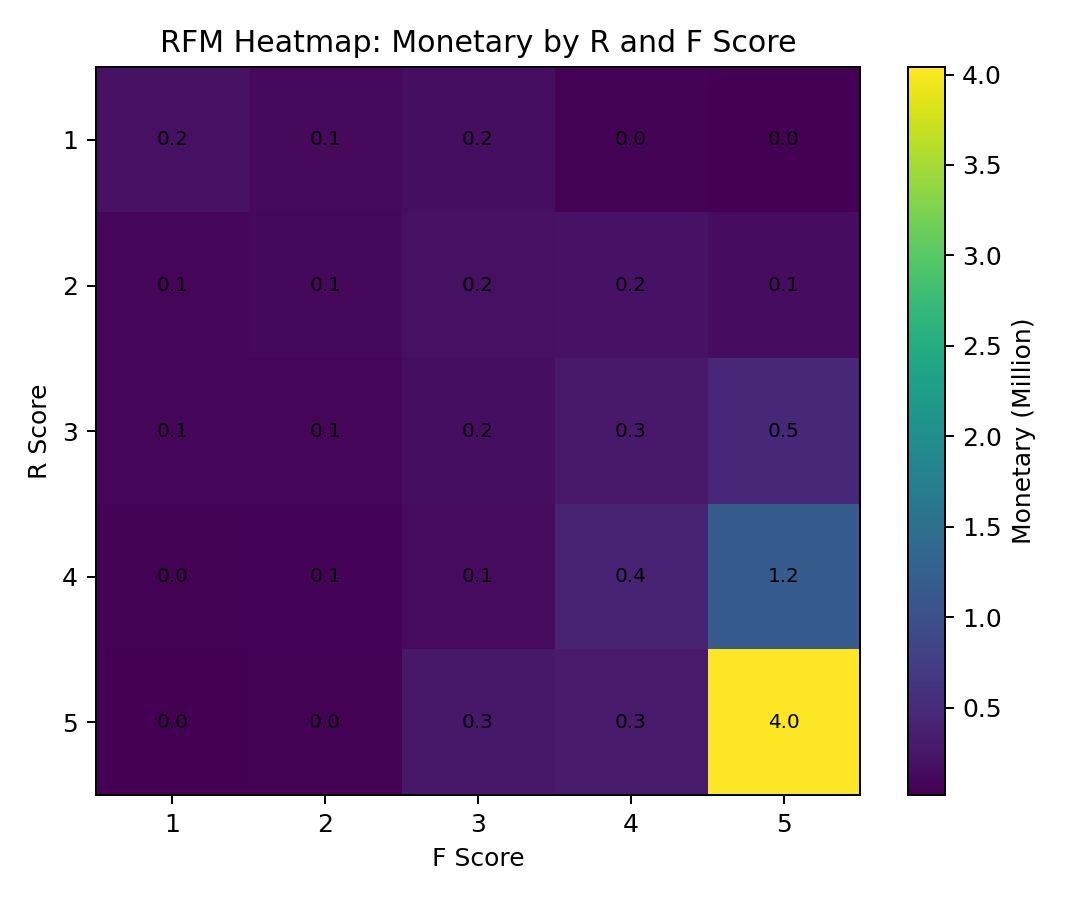
\includegraphics[width=0.72\textwidth]{figures/rfm_heatmap.png}
\caption{RFM Heatmap theo Monetary}
\sourceNote{Tính toán từ \texttt{tableau\_rfm\_segmentation.csv}}
\end{figure}

Heatmap cho thấy khu vực R\_Score cao và F\_Score cao có Monetary lớn nhất. Đây là vùng Champions/Loyal Customers. Ngược lại, vùng R\_Score thấp phản ánh khách hàng lâu chưa quay lại. Nếu F\_Score và M\_Score vẫn cao, đó là nhóm At Risk High Value cần ưu tiên chiến dịch win-back.

\section{Actionable Recommendations}

\subsection{Ưu tiên chiến lược theo segment}

\begin{longtable}{p{3.2cm}p{3.2cm}p{4.8cm}p{3.8cm}}
\caption{Action plan theo customer segment}\\
\toprule
\textbf{Segment} & \textbf{Vấn đề / cơ hội} & \textbf{Recommended action} & \textbf{KPI theo dõi} \\
\midrule
\endfirsthead
\toprule
\textbf{Segment} & \textbf{Vấn đề / cơ hội} & \textbf{Recommended action} & \textbf{KPI theo dõi} \\
\midrule
\endhead
Champions & Doanh thu cao, mua gần đây, tần suất cao & VIP loyalty program, early access, quà tặng theo tier, chăm sóc cá nhân hóa & Repeat purchase rate, retention rate, revenue per customer \\
Loyal Customers & Có tiềm năng tăng giá trị đơn hàng & Cross-sell, bundle, personalized product recommendation & AOV, conversion rate, attach rate \\
New Customers & Mới mua, chưa hình thành thói quen & Voucher cho đơn thứ hai trong 14-30 ngày, onboarding email sequence & Second purchase rate, time to second order \\
At Risk High Value & Giá trị cao nhưng lâu chưa quay lại & Win-back campaign ưu tiên, ưu đãi mạnh hơn, gọi lại/CSKH nếu phù hợp & Reactivation rate, recovered revenue, campaign ROI \\
At Risk & Có dấu hiệu giảm tương tác & Reminder email, remarketing, ưu đãi vừa phải & Open rate, click-through rate, reactivation rate \\
Lost Customers & Khả năng quay lại thấp & Low-cost remarketing, không ưu tiên ngân sách cao & Cost per recovered customer \\
Standard & Nhóm trung bình, quy mô lớn & Promotion định kỳ, product education, nurture campaign & Repeat rate, AOV, churn rate \\
\bottomrule
\end{longtable}

\subsection{Recommendation theo thị trường}

\begin{itemize}
    \item \textbf{Bảo vệ thị trường UK}: vì UK chiếm hơn 82\% doanh thu, cần có dashboard theo dõi riêng cho UK gồm churn rate, top products và repeat purchase rate.
    \item \textbf{Mở rộng thị trường phụ}: Germany, France, Netherlands và EIRE có doanh thu đứng sau UK. Nên chạy pilot campaign theo từng thị trường và đo CPA, AOV, retention.
    \item \textbf{Giảm rủi ro phụ thuộc}: đặt KPI tăng share doanh thu ngoài UK theo quý, ví dụ tăng non-UK revenue share từ khoảng 18\% lên 22-25\%.
\end{itemize}

\subsection{Recommendation theo sản phẩm}

\begin{itemize}
    \item Với sản phẩm có doanh thu cao và số đơn lớn: ưu tiên tồn kho, bundling, cross-sell.
    \item Với sản phẩm doanh thu cao nhưng số đơn thấp: kiểm tra outlier trước khi dự báo.
    \item Với sản phẩm bán chạy ở UK: thử nghiệm ở Germany/France để mở rộng thị trường.
\end{itemize}

\section{Dashboard Improvement Plan}

\begin{table}[H]
\centering
\caption{Checklist cải thiện dashboard trước khi nộp}
\begin{tabularx}{\textwidth}{p{4.2cm}p{5.8cm}X}
\toprule
\textbf{Hạng mục} & \textbf{Vấn đề hiện tại} & \textbf{Cách sửa} \\
\midrule
Segment Percent & Viz Extension không export được sang PDF & Thay bằng bar chart \% customers by segment hoặc native donut chart. \\
Chart title & Một số title chưa chuẩn hoặc lỗi ký tự & Chuẩn hóa: \textit{Top 10 Products by Revenue}, \textit{Sales by Customer Segment}. \\
Recommendation & Chưa có action panel rõ ràng & Thêm text box cuối dashboard: Key Insights \& Actions. \\
Bảng cuối & Có nhiều số, ít định hướng hành động & Thêm cột Business Action và Risk Priority. \\
Màu sắc & Segment có thể chưa thống nhất ý nghĩa & Dùng xanh cho tốt, xám cho standard, cam/đỏ cho rủi ro. \\
Layout & Dashboard dài nhưng cần khoảng cách đều & Dùng vertical/horizontal containers, tiled layout, padding 12-16 px. \\
\bottomrule
\end{tabularx}
\end{table}

\section{Technical Reproducibility}

\subsection{Cấu trúc thư mục nộp bài đề xuất}

\begin{lstlisting}[language=bash]
MCNA_DA_Intern_Test_Pham_Dinh_Duoc/
├── 01_Data/
│   ├── raw/data.csv
│   └── processed/
│       ├── tableau_transactions_final.csv
│       └── tableau_rfm_segmentation.csv
├── 02_SQL/ecommerce_analysis.sql
├── 03_Python/
│   ├── src/
│   │   ├── data_cleaning.py
│   │   ├── rfm_segmentation.py
│   │   ├── generate_tableau_data.py
│   │   └── main.py
│   └── requirements.txt
├── 04_Dashboard/
│   ├── dashboard.pdf
│   ├── dashboard.png
│   ├── dashboard.twbx
│   └── tableau_public_link.txt
├── 05_Slide/MCNA_DA_Test_Pham_Dinh_Duoc.pdf
├── 06_Video/MCNA_DA_Test_Pham_Dinh_Duoc.mp4
└── README.md
\end{lstlisting}

\subsection{Cách chạy pipeline}

\begin{lstlisting}[language=bash]
# From project root
python src/main.py

# Optional
python src/main.py --raw data/raw/data.csv --out data/processed --churn-days 180
\end{lstlisting}

\subsection{SQL validation examples}

\begin{lstlisting}[language=SQL]
-- Validate basic KPI
SELECT
    COUNT(*) AS total_rows,
    COUNT(DISTINCT InvoiceNo) AS total_orders,
    COUNT(DISTINCT CustomerID) AS total_customers,
    SUM(Sales) AS total_sales,
    SUM(Sales) / COUNT(DISTINCT InvoiceNo) AS aov
FROM transactions;

-- Monthly sales performance
SELECT
    STRFTIME('%Y-%m', InvoiceDate) AS month,
    SUM(Sales) AS total_sales,
    COUNT(DISTINCT InvoiceNo) AS total_orders,
    SUM(Sales) / COUNT(DISTINCT InvoiceNo) AS aov
FROM transactions
GROUP BY STRFTIME('%Y-%m', InvoiceDate)
ORDER BY month;

-- Top countries by sales
SELECT
    Country,
    SUM(Sales) AS total_sales,
    COUNT(DISTINCT InvoiceNo) AS total_orders,
    COUNT(DISTINCT CustomerID) AS total_customers
FROM transactions
GROUP BY Country
ORDER BY total_sales DESC
LIMIT 10;
\end{lstlisting}

\section{Limitations and Next Steps}

\subsection{Limitations}

\begin{itemize}
    \item \textbf{Attribution limitation}: dữ liệu hiện tại là transaction data, chưa có dữ liệu marketing campaign nên chưa thể đo hiệu quả từng kênh quảng cáo.
    \item \textbf{Profitability limitation}: chỉ có Sales, chưa có cost/margin nên chưa đánh giá được lợi nhuận theo sản phẩm hoặc segment.
    \item \textbf{Churn definition}: churn đang dựa trên Recency threshold; trong thực tế nên hiệu chỉnh threshold theo chu kỳ mua hàng của từng ngành/sản phẩm.
    \item \textbf{Product outlier}: một số sản phẩm có doanh thu cao bất thường từ rất ít đơn; cần kiểm tra bulk order trước khi khuyến nghị tồn kho.
    \item \textbf{January 2025}: dữ liệu tháng 1/2025 có thể chưa đủ tháng, nên không so sánh trực tiếp với tháng 12/2024 nếu không chuẩn hóa số ngày.
\end{itemize}

\subsection{Next Steps}

\begin{enumerate}
    \item Bổ sung margin/cost để chuyển từ Sales dashboard sang Profitability dashboard.
    \item Bổ sung campaign source để đo ROI của retention và remarketing.
    \item Tạo cohort analysis theo tháng mua đầu tiên để đo retention curve.
    \item Tạo customer-level action list cho nhóm At Risk High Value.
    \item Thiết lập dashboard refresh định kỳ và kiểm tra KPI hàng tuần.
\end{enumerate}

\section{Conclusion}

Dự án đã chuyển dữ liệu giao dịch e-commerce thành một hệ thống phân tích có tính hành động. Kết quả quan trọng nhất là sự tập trung doanh thu vào nhóm High-Value/Champions: khoảng 20\% khách hàng tạo gần 75\% doanh thu. Điều này cho thấy chiến lược tăng trưởng không nên chỉ tập trung vào acquisition mà cần đầu tư có chọn lọc vào retention.

Với dashboard hoàn thiện, doanh nghiệp có thể dùng báo cáo này để:

\begin{itemize}
    \item Theo dõi sức khỏe doanh thu và đơn hàng theo tháng.
    \item Xác định thị trường và sản phẩm chủ lực.
    \item Phân loại khách hàng theo RFM.
    \item Ưu tiên ngân sách retention cho nhóm có giá trị cao.
    \item Chuyển insight thành campaign cụ thể: VIP, win-back, second-order incentive và cross-sell.
\end{itemize}

\newpage
\appendix
\section{Appendix A: Tableau Calculated Fields}

\subsection{AOV}
\begin{lstlisting}
SUM([Sales]) / COUNTD([InvoiceNo])
\end{lstlisting}

\subsection{Churn Rate}
\begin{lstlisting}
COUNTD(IF [Status] = "Churned" THEN [CustomerID] END)
/
COUNTD([CustomerID])
\end{lstlisting}

\subsection{Segment Name}
\begin{lstlisting}
IF [R_Score] >= 4 AND [F_Score] >= 4 AND [M_Score] >= 4 THEN "Champions"
ELSEIF [R_Score] >= 4 AND [F_Score] >= 3 AND [M_Score] >= 3 THEN "Loyal Customers"
ELSEIF [R_Score] >= 4 AND [F_Score] <= 2 THEN "New Customers"
ELSEIF [R_Score] <= 2 AND [F_Score] >= 4 AND [M_Score] >= 4 THEN "At Risk High Value"
ELSEIF [R_Score] <= 2 AND [F_Score] >= 3 THEN "At Risk"
ELSEIF [R_Score] <= 2 AND [F_Score] <= 2 THEN "Lost Customers"
ELSE "Standard"
END
\end{lstlisting}

\section{Appendix B: Recommended Slide Storyline}

\begin{enumerate}
    \item Title: E-Commerce Sales \& Customer Retention Analytics.
    \item Business context: doanh nghiệp cần hiểu revenue drivers và churn risk.
    \item Data pipeline: SQL $\rightarrow$ Python $\rightarrow$ Tableau $\rightarrow$ Recommendation.
    \item KPI summary: Sales, Orders, AOV, Customers, Churn Rate.
    \item Revenue insight: Q4 peak và mùa vụ.
    \item Market/product insight: UK dominance và top products.
    \item RFM insight: Champions và At Risk High Value.
    \item Key insight: Top 20\% customers contribute nearly 75\% revenue.
    \item Action plan: VIP, win-back, second purchase, cross-sell.
    \item Closing: từ dashboard tới decision system.
\end{enumerate}

\end{document}
